\documentclass{article} % For LaTeX2e
\usepackage{nips13submit_e,times}
\usepackage{hyperref}
\usepackage{url}
\usepackage[pdftex]{graphicx} 
\usepackage{listings}
%\documentstyle[nips13submit_09,times,art10]{article} % For LaTeX 2.09


\title{Formatting Instructions for NIPS 2013}


\author{
Jiarong Ye \\
College of Engineering\\
College of Eberly Science\\
The Pennsylvania State University\\
State College, PA 16801 \\
\texttt{jxy225@psu.edu} \\
}


\newcommand{\fix}{\marginpar{FIX}}
\newcommand{\new}{\marginpar{NEW}}

\nipsfinalcopy 

\begin{document}


\maketitle

\begin{abstract}
A one paragraph summary of what is the goal of the project, and what are the findings. It should summarize the entire report.
\end{abstract}

\section{Introduction}



Introducing the research problem and related specific research hypotheses 




\section{Data set}


Describe in details about the data: how the data was collected and the variables in the data set.

\section{Exploratory data analysis}

Look at the data univariately/multivariately with figures and/or numerical sum- maries. Describe your results.



\section{Modeling}


\subsection{Description}
Start by building the model based on the previous exploratory data analysis. Address the research questions when designing the model, and justify your choice of the model. Specifically, you should discuss how you carried out the steps in analysis. Final model: Summarize your final model. Give interpretations based on the model in the context of the problem.


List all sources of variation you can think of in the response variable, including treatment factors and their levels, experimental units, noise factors, and covariates.


Decide how many experimental units you can analyze, and determine how you will assign treatments to the experimental units (Completely randomized design?  Blocking factors? )


\subsection{Data Model}
Write out the model you will fit with the collected data




\section{Results}

Address all the specific research questions.

Summarize the results of your experiment briefly, and note anything that could have made the experiment better.

\section{Conclusion}

What are you conclusions? What are the key findings, and discuss, with reference to the supporting information. Any possible explanations associated with your findings? E.g, how would you explain the patterns you find? Any limitations if your study? Any possible improvement to your analysis?



\begin{figure}[h]
\begin{center}
%\framebox[4.0in]{$\;$}
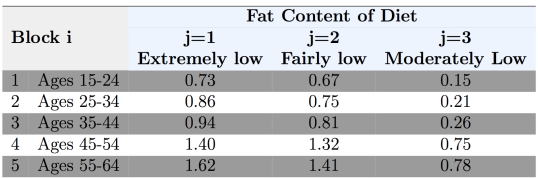
\includegraphics[height=4cm, width=12cm]{1.png}
\end{center}
\caption{Sample figure caption.}
\end{figure}

\subsection{Tables}

(except for first word and proper nouns); tables are numbered consecutively.

\begin{table}[t]
\caption{Sample table title}
\label{sample-table}
\begin{center}
\begin{tabular}{ll}
\multicolumn{1}{c}{\bf PART}  &\multicolumn{1}{c}{\bf DESCRIPTION}
\\ \hline \\
Dendrite         &Input terminal \\
Axon             &Output terminal \\
Soma             &Cell body (contains cell nucleus) \\
\end{tabular}
\end{center}
\end{table}


 


\bibliographystyle{plain}
\bibliography{ref}


\section{Appendix}

\appendix

\lstset{language=R}
\lstset{frame=lines}
\lstset{caption={Split data into training and validation dataset}}
\lstset{basicstyle=\footnotesize}
\begin{lstlisting}
treatments.not.random=c(rep("1",10), rep("2",10), rep("3", 10))
treatment=sample(treatments.not.random)
experiment_unit = 1:length(treatment)
table=data.frame(experiment_unit, treatment,row.names=NULL)
table
\end{lstlisting}


\end{document}
